\documentclass{artikel3}

\usepackage{pslatex,graphicx,amsmath,amssymb}
\usepackage{pdflatex}

\newtheorem{theorem}{Theorem}

\newcounter{excounter}
\newenvironment{exercise}
  {\refstepcounter{excounter}
   \begin{quotation}\textbf{Exercise \arabic{excounter}.} }
  {\end{quotation}}

\begin{document}
\title{SSC 335: demo}
\author{Victor Eijkhout}
\date{today}
\maketitle

\section{This is a section}
\label{sec:intro}

This is a test document, used in~\cite{latexdemo}. It contains a
discussion in section~\ref{sec:discussion}.

\begin{exercise}\label{easy-ex}
  Left to the reader.
\end{exercise}
\begin{exercise}
  Also left to the reader, just like in exercise~\ref{easy-ex}
\end{exercise}

\begin{theorem}
  This is cool.
\end{theorem}
This is a formula: $a\Leftarrow b$.
\begin{equation}
  \label{eq:one}
    x_i\leftarrow y_{ij}\cdot x^{(k)}_j
\end{equation}
Text: $\int_0^1 \sqrt x\,dx$
\[
  \int_0^1 \sqrt x\,dx
\]
\section{This is another section}
\label{sec:discussion}

\begin{table}[ht]
  \centering
  \begin{tabular}{|rl|}
    \hline one&value \\ \hline another&values \\ \hline
  \end{tabular}
  \caption{This is the only table in my demo}
  \label{tab:thetable}
\end{table}
\begin{figure}[ht]
  \centering
  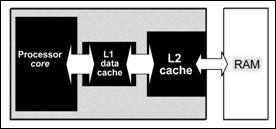
\includegraphics{graphics/caches}
  \caption{this is the only figure}
  \label{fig:thefigure}
\end{figure}
As I showed in the introductory section~\ref{sec:intro}, in the
paper~\cite{AdJo:colorblind}, it was shown that
equation~\eqref{eq:one}
\begin{itemize}
\item There is an item.
\item There is another item
  \begin{itemize}
  \item sub one
  \item sub two
  \end{itemize}
\end{itemize}
\begin{enumerate}
\item item one
\item item two
  \begin{enumerate}
  \item sub one
  \item sub two
  \end{enumerate}
\end{enumerate}

\tableofcontents
\listoffigures

\bibliography{math}
\bibliographystyle{plain}

\end{document}
